\chapter{Resultados} \label{chap:resultados}

\section{Cinemática Directa}
Utilizando la Tabla DH, y el código de Cinemática Directa, se hace un diagrama en Matlab, para confirmar la geometría del robot.
\begin{figure}[H]
    \centering
    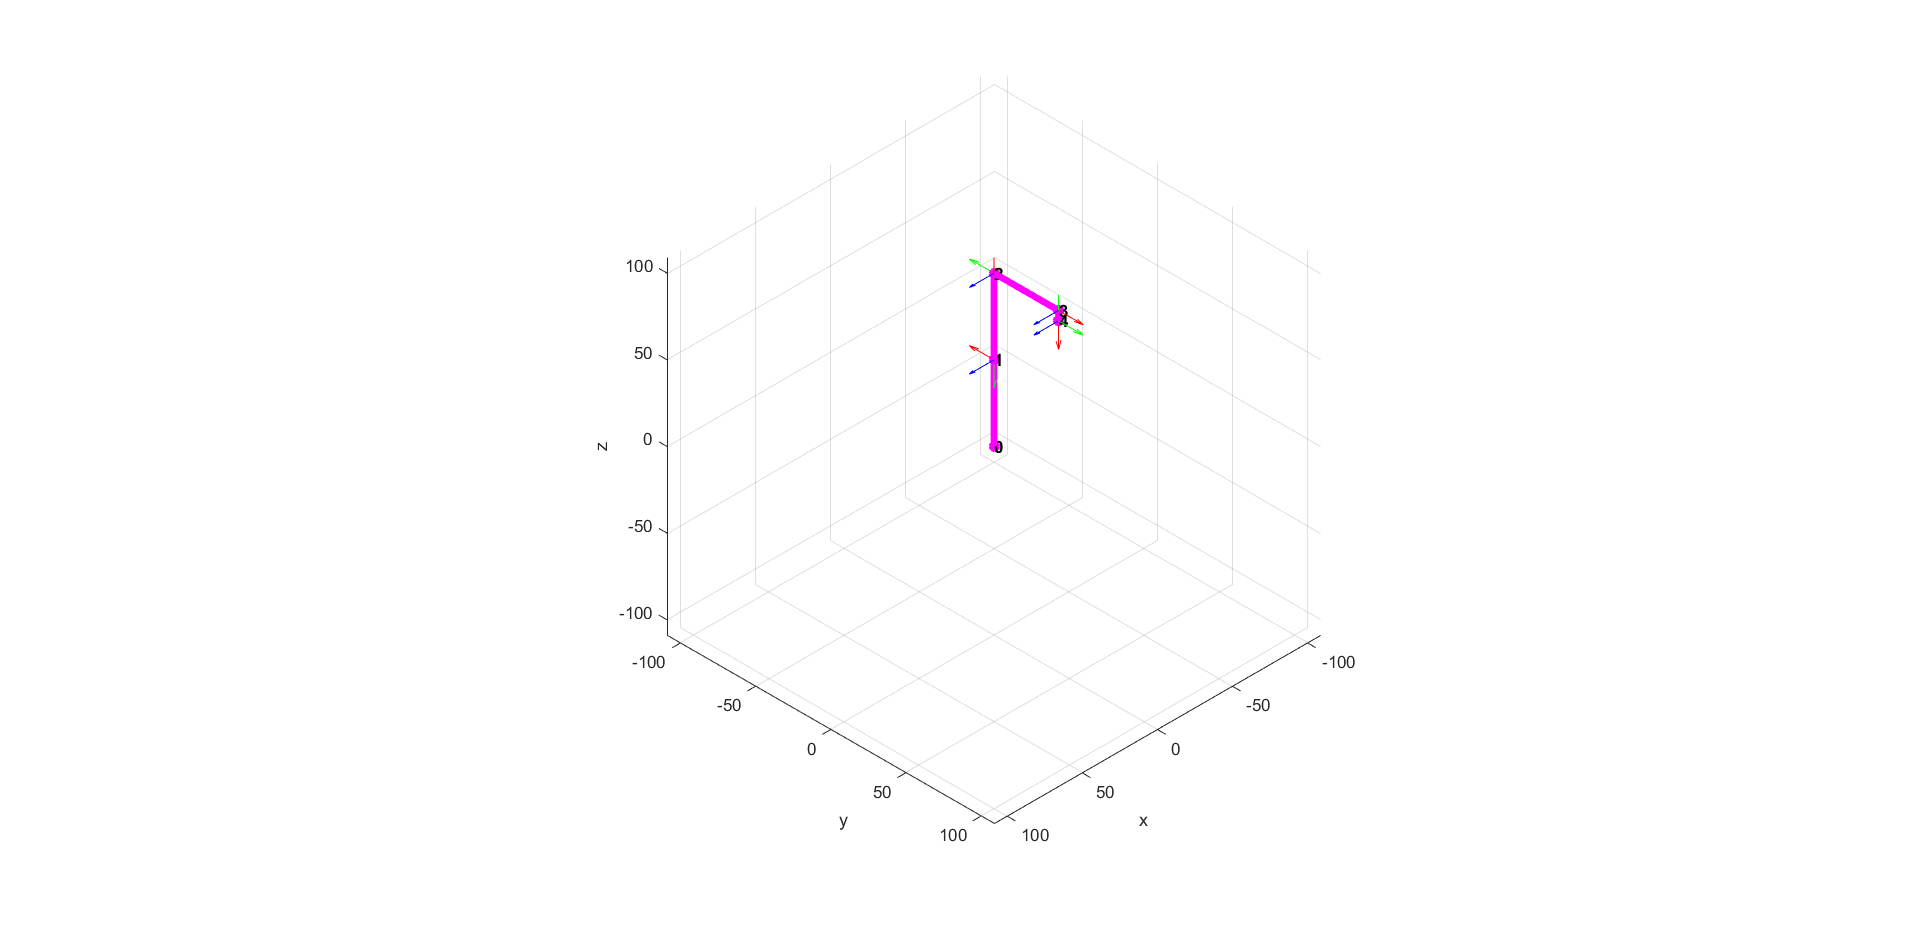
\includegraphics[width=1\textwidth]{img/robotFinal_DH.png}
    \caption{Prueba DH Robot}
    \label{fig:pruebaDH_robot}
\end{figure}
El dibujo creado concuerda con el diagrama de Denavit Hartenberg y con el modelo 3D del robot en Solidworks, por lo tanto se definieron los parametros y características correctamente.

\section{Cinemática Diferencial}
Las siguientes gráficas representan el cambio de posición, velocidad y aceleración del efector final respecto al tiempo. En la parte superior, la posición muestra la trayectoria en los ejes X, Y y Z; como se puede observar, se presenta una trayectoria de tipo sinusoidal o cosenoidal. En la gráfica de la velocidad lineal, las curvas indican cambios bruscos de dirección, aceleraciones y desaceleraciones a lo largo del tiempo. Por último, la aceleración indica variaciones rápidas de velocidad, es decir, aceleraciones intensas.

En la segunda parte, se muestra la orientación del efector final en coordenadas de Euler, donde $\phi$ representa la rotación en X, $\theta$ rotación en Y, y $\theta$ rotación en Z. La velocidad angular presenta la rapidez de cambio de los ángulos y la aceleración indica los cambios en la velocidad angular, útil para estimar esfuerzos dinámicos. 

\begin{figure}[H]
    \centering
    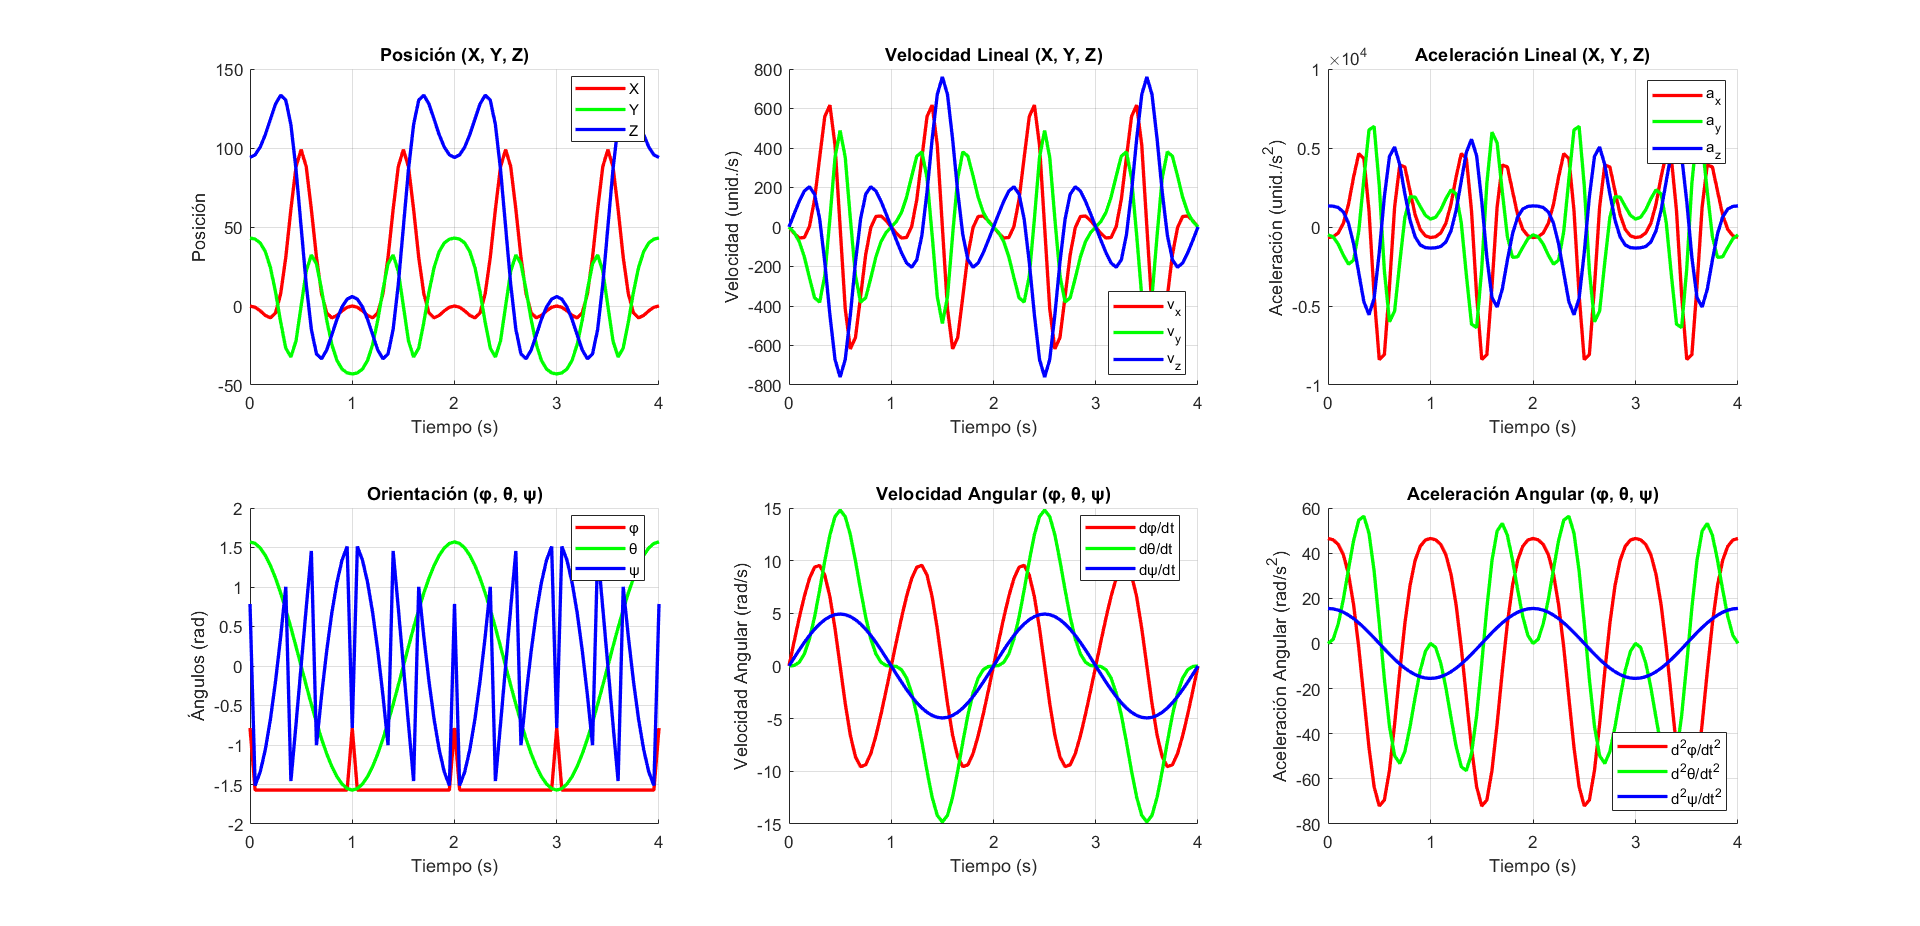
\includegraphics[width=1\textwidth]{img/graficas_diferencial.png}
    \caption{Gráficas Cinemática Diferencial}
    \label{fig:grafica_diferencial}
\end{figure}